%Zeitz auskommentiert   \begin{center}                    
%                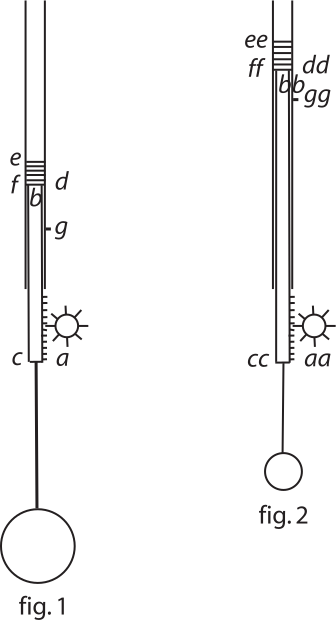
\includegraphics[width=0.35\textwidth]{images/37_4_113r}
%                        %\caption{Bildbeschreibung}
%                        \end{center}
                        \pstart[113 v\textsuperscript{o}]  \edlabel{113desc}\textso{Exper. 3.} Cujuscunque vero crassitiei aut etiam heterogeneitatis pondera sint, semper tantundem ponderis supra quodcunque assumtum in linea descensus punctum, relinquetur. Esto in fig. 1. punctum assumtum \textit{c}. Quantumcunque augeatur pondus quod extabit supra \textit{c} \edlabel{113vdesc}
%Fussnote mit der vorherigen zusammengefasst
%\edtext{}{\lemma{descensu.}\xxref{1132desc}{113vdesc}\Afootnote{ \textit{ (1) }\ \textso{Exp. 3.}  \textit{(a)}\ Ideo generaliter quantaecunque  \textit{(aa)}\ sit crassitiei pondus\protect\index{Sachverzeichnis}{pondus|textit} incumbens \textit{(bb)}\ crassitiei aut altitudinis pondera incumbentia sint  \textit{(aaa)}\ semper manebit in spatio \textit{(bbb)}\ extabit ultra in altitudine quacunque ex \textit{d}  \textit{(aaaa)}\ pondus\protect\index{Sachverzeichnis}{pondus|textit} minus altum \textit{(bbbb)}\ pondus\protect\index{Sachverzeichnis}{pondus|textit} altitudinis minoris  \textit{(aaaaa)}\ praevaleat \textit{(bbbbb)}\ aequivaleat \textit{(b)}\ Quod si vero crassities non sit eadem, aut pondera non sint homogenea, tunc semper manebit supra \textit{c} \textit{ (2) }\  \textso{Exper. 3.} [...] sint, \textit{(a)}\ quantum \textit{(b)}\ semper tantundem  \textit{(aa)}\ inter \textit{(bb)}\ supra quodcunque assumtum descensus pondus\protect\index{Sachverzeichnis}{pondus|textit} \textit{(cc)}\ ponderis [...] \textit{c} \textit{ L}}}
 semper aequiponderabit columnae \textit{cd}. Quia hoc \edtext{solum pondus \textit{dc} aut ei aequale sustentando}{\lemma{hoc}\Afootnote{ \textit{ (1) }\ solo sustentato \textit{ (2) }\ solum [...] sustentando \textit{ L}}}, omnem vim suam residuam (si \edtext{scilicet}{\lemma{}\Afootnote{scilicet \textit{ erg.} \textit{ L}}} ea pondera quae jam infra \textit{c} forsan esse Elateriumque\protect\index{Sachverzeichnis}{elaterium} premere possunt adimas) \edtext{impendit}{\lemma{adimas)}\Afootnote{ \textit{ (1) }\ consumit \textit{ (2) }\ impendit \textit{ L}}}. Non ergo demittit unquam hoc pondus eive aequalens, etsi caetera omnia superfusa adjectave sine resistentia demittat; id est demittet totum infra \textit{dc} quantumcunque sit demta \edtext{tantum praecise}{\lemma{demta}\Afootnote{ \textit{ (1) }\ quo \textit{ (2) }\ tantum praecise \textit{ L}}} parte quadam columnae \textit{fc} aequiponderante\edlabel{aequi113a}\edtext{}{\lemma{}\xxref{aequi113a}{aequi113b}\Afootnote{aequiponderante  \textbar\ , quantamcunque sit totum \textit{ gestr.}\ \textbar\ . \textso{Exper. 4} \textit{ L}}}.
 \pend 
%zeitz auskommentiert          \begin{center}                    
%                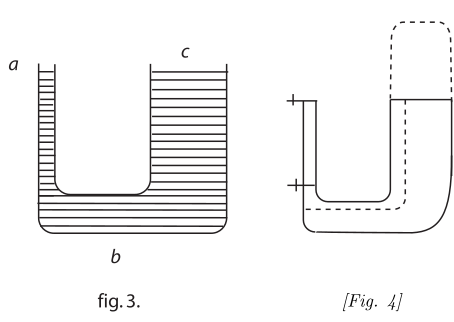
\includegraphics[width=0.7\textwidth]{images/37_4_113v_2_3}
%                        %\caption{Bildbeschreibung}                      
%                        %@ @ @ Dies ist eine Abstandszeile - fuer den Fall, dass mehrere figures hintereinander kommen, ohne dass dazwischen laengerer Text steht. Dies kann zu einer Fahlermeldung fuehren. @ @ @ \\
%                 %  \begin{wrapfigure}{l}{0.2\textwidth}                    
%             %   \includegraphics[width=0.28\textwidth]{images/37_4_113v_2}\\\textit{[Fig. 4]}
%                \end{center}
%                        %\caption{Bildbeschreibung}
%                     %   \end{wrapfigure}
%                        %@ @ @ Dies ist eine Abstandszeile - fuer den Fall, dass mehrere figures hintereinander kommen, ohne dass dazwischen laengerer Text steht. Dies kann zu einer Fahlermeldung fuehren. @ @ @ \\
                        \pstart\textso{Exper. 4.}  \edlabel{aequi113b}Si Elaterium\protect\index{Sachverzeichnis}{elaterium} pariter et pondus\protect\index{Sachverzeichnis}{pondus} liquida sint nec Elaterii\protect\index{Sachverzeichnis}{elaterium},
                         nec ponderis\protect\index{Sachverzeichnis}{pondus} \edtext{altitudo crassitiesve sed species tantum}{\lemma{ponderis}\Afootnote{ \textit{ (1) }\ crassities ponderis\protect\index{Sachverzeichnis}{pondus|textit} \textit{ (2) }\ altitudo crassitiesve sed species tantum \textit{ L}}} altitudinem suspensionis \edtext{variat. Species}{\lemma{variat.}\Afootnote{ \textit{ (1) }\ Sed sola species Elaterii\protect\index{Sachverzeichnis}{elaterium|textit} \textit{ (2) }\ Species \textit{ L}}} inquam, id est si pondus\protect\index{Sachverzeichnis}{pondus} sit aqua aut Mercurius\protect\index{Sachverzeichnis}{mercurius}, si Elaterium\protect\index{Sachverzeichnis}{elaterium} sit aer rarus aut compressus, quae specie variare dico quia pari magnitudine et \edtext{figura externisque omnibus}{\lemma{figura}\Afootnote{ \textit{ (1) }\ alii \textit{ (2) }\ externisque omnibus \textit{ L}}} diversos tamen exercent effectus. Ratio est, quia \edtext{Liquores}{\lemma{quia}\Afootnote{ \textit{ (1) }\ in liquoribus\protect\index{Sachverzeichnis}{liquor|textit} crassities \textit{ (2) }\ Liquores \textit{ L}}} neque ponderant neque vim Elasticam\protect\index{Sachverzeichnis}{vis!elastica} in vim aliam oppositam exercent, secundum crassitiem,  dudum in Hydrostaticis\protect\index{Sachverzeichnis}{hydrostatica} demonstratum est liquores\protect\index{Sachverzeichnis}{liquor} non pondere secundum crassitiem Tuborum vasorumque quia liquor\protect\index{Sachverzeichnis}{liquor} magis arctatus celerius movetur inspice fig. 3.  Ubi sipho\protect\index{Sachverzeichnis}{sipho} bicrurus cruribus sursum spectantibus apertisque
                    diversae capacitatis \edtext{ liquore}{\lemma{capacitatis}\Afootnote{ \textit{ (1) }\ aqua \textit{ (2) }\  liquore \textit{ L}}} \edtext{quodam homogeneo}{\lemma{liquore}\Afootnote{ \textit{ (1) }\ eo \textit{ (2) }\ quodam homogeneo \textit{ L}}} plenus cogitetur. Constat,    
                   et a Stevino\protect\index{Namensregister}{\textso{Stevin} (Stevinus), Simon 1548\textendash 1620} aliisque dudum ostensum est, etsi in tubo arctiore \textit{ab} minus sit aquae quam in ampliore [\textit{bc}]\edtext{}{\Afootnote{\textit{b}\textit{\ L \"{a}ndert Hrsg. } }} attamen minorem majori aequiponderare, dummodo eadem sit tuborum altitudo. Ratio est, quia angustia tubi quantum adimit materiae, tantum addit motui, necesse est enim aquam\edtext{}{\lemma{}\Afootnote{aquam  \textbar\ \textit{cd} \textit{streicht Hrsg.}\ \textbar\ per \textit{ L}}} per tubum \textit{bc} exituram celerrime moveri sursum, dum ipsa tarde descendit in Tubo \textit{bc}. Est enim generale omnium machinarum principium, ut celeritate motus materia compensetur. Cum ergo hoc principium generale locum habeat, sive \edtext{per pondus sive per Elaterium depressus ex crure \textit{cb} transeat in crus \textit{ba}}{\lemma{sive}\Afootnote{ \textit{ (1) }\ per pondus sive per Elaterium\protect\index{Sachverzeichnis}{elaterium|textit} liquor\protect\index{Sachverzeichnis}{liquor|textit} \textit{cb} tendat in vas ex \textit{(a)}\ tubo \textit{(b)}\ crure \textit{cb} \textit{ (2) }\ per pondus sive per Elaterium  \textit{(a)}\ liquor\protect\index{Sachverzeichnis}{liquor|textit} ex tubo \textit{cb} \textit{(b)}\ depressus [...] \textit{ba} \textit{ L}}} semper enim liquor\protect\index{Sachverzeichnis}{liquor} in \textit{ab} tanto celerius movebitur, quam in \textit{cb} quanto crus ipsum 